\documentclass{oci}
\usepackage[utf8]{inputenc}
\usepackage{lipsum}
\usepackage{tikz}
\usepackage{pgfplots}
\usetikzlibrary{shapes.misc}

\tikzset{cross/.style={cross out, draw=black, inner sep=0pt, outer sep=0pt},
%default radius will be 1pt.
cross/.default={1pt}}

\title{El juego del calendario}

\begin{document}
\begin{problemDescription}
  Alicia acaba de inventar un juego muy particular.
  Para poder jugarlo solo se necesita un lápiz y el calendario de un mes de 30 días.
  Los días del mes se numeran de 1 a 30 y dependiendo del mes, el primer día puede caer
  en distintos días de la semana.
  Por ejemplo, la siguiente imagen muestra el calendario de un mes donde el primer día cae un viernes.
  \begin{center}
    \scalebox{0.8}{
      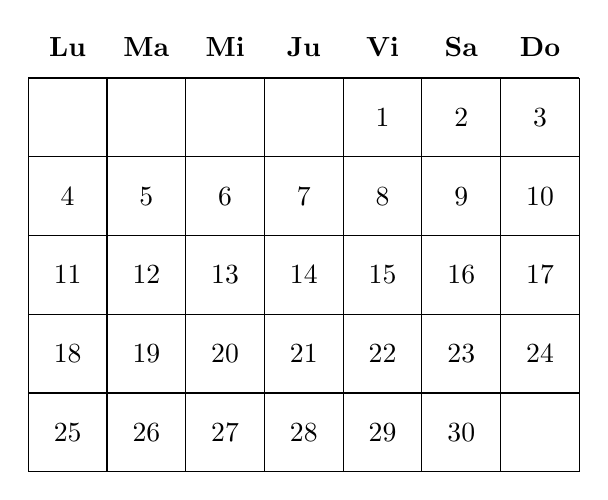
\begin{tikzpicture}
        \draw (0, 0) grid (7, 5);
        \def\weeks{5}
        \def\start{4}
        \foreach \d [count=\x from 0] in {Lu, Ma, Mi, Ju, Vi, Sa, Do}{
          \node at (\x + 0.5, \weeks + 0.4) {\textbf{\d}};
        };
        \foreach \i in {0, ..., 29}{
          \pgfmathtruncatemacro{\x}{Mod(\start + \i, 7)}
          \pgfmathtruncatemacro{\y}{(\start + \i) / 7}
          \pgfmathtruncatemacro{\d}{\i + 1}
          \node[fill=white] at (\x + 0.5, \weeks - \y - 0.5) {\d};
        }
      \end{tikzpicture}
    }
  \end{center}

  El juego comienza escogiendo un día inicial $x$, el cual debe ser tachado inmediatamente
  marcándolo como visitado.
  Posteriormente, en cada paso hay que aplicar una regla que indica el siguiente día al que hay
  que moverse el cual debe ser tachado marcándolo como visitado.
  El juego termina cuando una regla indica que hay que moverse a un día que ya había sido tachado
  o cuando no es posible aplicar una regla.
  La regla que hay que aplicar en cada paso depende del día de la semana en que cae el día actual.
  Las reglas para cada día de la semana se detallan a continuación:
  \begin{itemize}
   \item[\bf Lunes] Avanzar de uno en uno hasta encontrar el primer día no tachado y moverse a este día.
    Si al avanzar buscando un día sin tachar se llega al final del mes se debe \emph{dar la vuelta} y
    continuar avanzando desde el inicio del mes.
    Si no queda ningún día sin tachar la regla no puede aplicarse y el juego termina en el día actual.

    \item[\bf Martes] Moverse al día que corresponde al \emph{reflejo} del día actual.
    Es decir, si el día actual es $i$ moverse al día $31 - i$.

    \item[\bf Miércoles] Si el día actual es par, moverse al día anterior.
    Si el día actual es impar, moverse al día siguiente.

    \item[\bf Jueves] Moverse al día que esta 10 posiciones adelante dando la vuelta en caso de
    llegar al final del mes.

    \item[\bf Viernes] Si el día actual $i$ es par, moverse al día $i/2$.
    En caso contrario, moverse al día $3\times i + 1$.
    Si $3\times i + 1$ es mayor que 30 restarle 30 al resultado hasta que este sea menor o igual que 30.

    \item[\bf Sábado] Si el día actual es $i$ moverse al día $2\times i$.
    Si $2\times i$ es mayor que 30 restarle 30 al resultado hasta que este sea menor o igual que 30.

    \item[\bf Domingo] Avanzar de dos en dos hasta encontrar un día no tachado y moverse a este día.
    Dar la vuelta al mes en caso de ser necesario.
    Si no puede avanzarse a ningún día sin tachar la regla no puede aplicarse y el juego termina en el día actual.
  \end{itemize}

  Considera el calendario del ejemplo mostrado anteriormente donde el primer día cae un viernes.
  Si escogemos el día inicial $x=16$ este cae un sábado.
  La regla para el sábado dice que hay que moverse al día $2\times 16 = 32$, como este es mayor que 30
  restamos 30 una vez y nos movemos al día 2.
  El día 2 cae un sábado nuevamente y por lo tanto nos movemos al día $2\times 2=4$.
  El día 4 cae un lunes.
  La regla del lunes dice que hay que encontrar el siguiente día no tachado el cual es el martes 5.
  La regla para el martes nos pide movernos al reflejo que en este caso corresponde al día $31 - 5 = 26$.
  El día 26 es nuevamente un martes y la regla nos pide movernos al día $31 - 5 = 5$ el cual ya había
  sido tachado y por lo tanto el juego termina en el día 5.
  La siguiente imagen muestra la secuencia de movimientos descritos anteriormente.

  \begin{center}
    \scalebox{0.8}{
      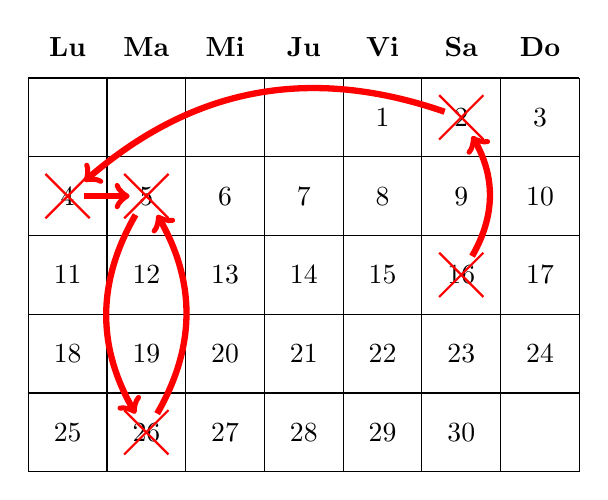
\begin{tikzpicture}
        \draw (0, 0) grid (7, 5);
        \def\weeks{5}
        \def\start{4}
        \foreach \d [count=\x from 0] in {Lu, Ma, Mi, Ju, Vi, Sa, Do}{
          \node at (\x + 0.5, \weeks + 0.4) {\textbf{\d}};
        };
        \foreach \i in {0, ..., 29}{
          \pgfmathtruncatemacro{\x}{Mod(\start + \i, 7)}
          \pgfmathtruncatemacro{\y}{(\start + \i) / 7}
          \pgfmathtruncatemacro{\d}{\i + 1}
          \node[fill=white] (\d) at (\x + 0.5, \weeks - \y - 0.5) {\d};
        }
        \node[cross, thick, red, minimum size=16] at (16) {};
        \node[cross, thick, red, minimum size=16] at (2) {};
        \node[cross, thick, red, minimum size=16] at (4) {};
        \node[cross, thick, red, minimum size=16] at (5) {};
        \node[cross, thick, red, minimum size=16] at (26) {};
        \draw[->,red, line width=0.8mm, bend right] (16) edge (2);
        \draw[->,red, line width=0.8mm, bend right] (2)  edge (4);
        \draw[->,red, line width=0.8mm]             (4)  edge (5);
        \draw[->,red, line width=0.8mm, bend right] (5)  edge (26);
        \draw[->,red, line width=0.8mm, bend right] (26) edge (5);
      \end{tikzpicture}
    }
  \end{center}

  Dado el día de la semana en que cae el primer día del mes y el día inicial $x$ con que comienza
  el juego tu tarea es determinar el día en que finaliza el juego.
\end{problemDescription}

\begin{inputDescription}
  La entrada contiene una línea con dos enteros $d$ ($0 \leq d \leq 6$) y $x$ ($1 \leq x \leq 30$).
  El entero $d$ corresponde al día de la semana en que cae el primer día del mes.
  Si $d$ es $0$ el mes comienza un lunes, si $d$ es $1$ el mes comienza un martes y así hasta el domingo.
  El entero $x$ indica el día del mes en que comienza el juego.
\end{inputDescription}

\begin{outputDescription}
  La salida debe contener un único entero indicando el día del mes en el que termina el juego.
\end{outputDescription}

\begin{scoreDescription}
  Este enunciado no contiene subtareas, se entregará puntaje proporcional a la cantidad de casos
  de prueba correctos siendo 100 el puntaje máximo.
  % \subtask{40}
  % Se probarán varios casos donde $d = 0$, es decir, el mes siempre comienza un lunes.
  % \subtask{60}
  % Se probarán varios casos sin restricciones adicionales.
\end{scoreDescription}

\begin{sampleDescription}
\sampleIO{sample-1}
\sampleIO{sample-2}
\end{sampleDescription}

\end{document}
